% Sistema de mano derecha vs mano izquierda (reflexión) — libro figs. 4.4, 4.6
\documentclass[border=5pt]{standalone}
\usepackage{tikz}
\usetikzlibrary{arrows.meta, calc}
\begin{document}
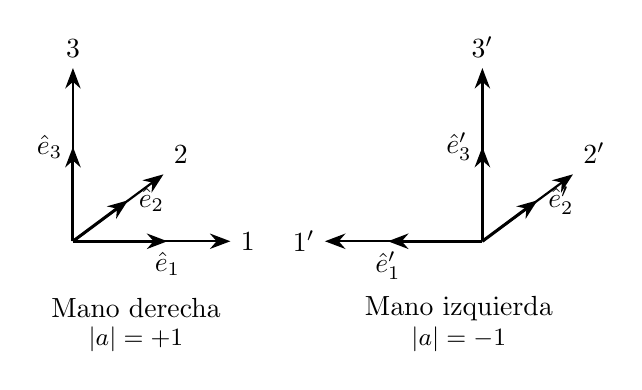
\begin{tikzpicture}[>={Stealth[length=2.6mm]}, line width=0.8pt]
  % ===== Mano derecha =====
  \begin{scope}
    \draw[->] (0,0)--(2.0,0) node[right]{$1$};
    \draw[->] (0,0)--(1.15,0.85) node[above right]{$2$};
    \draw[->] (0,0)--(0,2.2) node[above]{$3$};
    \draw[->, line width=1.1pt] (0,0)--(1.2,0) node[below]{$\hat e_1$};
    \draw[->, line width=1.1pt] (0,0)--(0.7,0.52) node[right]{$\hat e_2$};
    \draw[->, line width=1.1pt] (0,0)--(0,1.2) node[left]{$\hat e_3$};
    \node at (0.8,-0.85){Mano derecha};
    \node[font=\small] at (0.8,-1.25){$|a|=+1$};
  \end{scope}
  % ===== Mano izquierda (reflexión x_1 -> -x_1) =====
  \begin{scope}[xshift=5.2cm]
    \draw[->] (0,0)--(-2.0,0) node[left]{$1'$};
    \draw[->] (0,0)--(1.15,0.85) node[above right]{$2'$};
    \draw[->] (0,0)--(0,2.2) node[above]{$3'$};
    \draw[->, line width=1.1pt] (0,0)--(-1.2,0) node[below]{$\hat e'_1$};
    \draw[->, line width=1.1pt] (0,0)--(0.7,0.52) node[right]{$\hat e'_2$};
    \draw[->, line width=1.1pt] (0,0)--(0,1.2) node[left]{$\hat e'_3$};
    \node at (-0.3,-0.85){Mano izquierda};
    \node[font=\small] at (-0.3,-1.25){$|a|=-1$};
  \end{scope}
\end{tikzpicture}
\end{document}
